\documentclass{article}
\usepackage{amssymb}
\usepackage{changepage}
\usepackage{amsmath}
\usepackage{gensymb}
\usepackage{cancel}
\usepackage{tkz-euclide}
\usepackage{graphicx}
\title{Momentum and Energy Summary}
\author{Tristan Simpson}
\begin{document}
\maketitle

\section{Equations (1)}
\begin{adjustwidth}{1cm}{0pt}
    \subsection*{Energy without a spring}
    \begin{flushleft}
        If the object is moving at start, then the variable $E_{k}$ has a value. Else, if the object is not moving at start, set $E_{k}$ to zero.
    \end{flushleft}
    \begin{align*}
        E_{tot}                   & = E_{tot}\prime                              \\
        E_{k} + E_{g}             & = E_{k}\prime + E_{g}\prime                  \\
        (\frac{1}{2}mv^2) + (mgh) & = (\frac{1}{2}mv^2)\prime + (mgh)\prime &  &
    \end{align*}
    \vspace*{0.03cm}
    \subsection*{Energy with a spring}
    \begin{flushleft}
        If there is a force/object pushing on the spring, then the variable $E_{e}$ has a value. Else, it's value is zero. Therefore, if an object is being dropped onto a spring, only $E_{e}\prime$ has a value.
    \end{flushleft}
    \begin{align*}
        E_{tot}                                       & = E_{tot}\prime                                                        \\
        E_{k} + E_{g}     + E_{e}                     & = E_{k}\prime + E_{g}\prime  + E_{e}\prime                             \\
        (\frac{1}{2}mv^2) + (mgh) + (\frac{1}{2}kx^2) & = (\frac{1}{2}mv^2)\prime + (mgh)\prime + (\frac{1}{2}kx^2)\prime &  &
    \end{align*}
    \vspace*{0.03cm}
    \subsection*{Elastic Momentum}
    \begin{flushleft}
        The two objects do \textbf{\textit{not}} move together after colliding. Instead, they seperate from eachother, both going in different paths.
    \end{flushleft}
    \begin{align*}
        P_{tot}                         & = P_{tot}\prime                                    \\
        P_{a} + P_{b}                   & = P_{a}\prime + P_{b}\prime                        \\
        (m_{a})(v_{a}) + (m_{b})(v_{b}) & = (m_{a})(v_{a})\prime + (m_{b})(v_{b})\prime &  &
    \end{align*}
    \vspace*{0.03cm}
    \subsection*{Inelastic Momentum}
    \begin{flushleft}
        The two objects move together after colliding. Instead of seperating from eachother, the two objects have conjoined, both moving in the same path.
    \end{flushleft}
    \begin{align*}
        P_{tot}                         & = P_{tot}\prime                   \\
        P_{a} + P_{b}                   & = P_{ab}                          \\
        (m_{a})(v_{a}) + (m_{b})(v_{b}) & = (m_{a + b})(v_{a\times b}) &  &
    \end{align*}
\end{adjustwidth}

\section{Units}
\begin{adjustwidth}{1cm}{0pt}
    \begin{minipage}{0.33\textwidth}
        \begin{itemize}
            \item $F_{s} = N$
            \item $k = \frac{N_{ewtons}}{m_{eter}}$
            \item $x = m_{eters}$
            \item $P_{tot} = \frac{kgm}{s}$
        \end{itemize}
    \end{minipage}
    \begin{minipage}{0.33\textwidth}
        \begin{itemize}
            \item $E_{e} = J$
            \item $W = J$
            \item $\Delta E = J$
            \item $E_{tot} = J$
        \end{itemize}
    \end{minipage}
\end{adjustwidth}

\vspace*{0.5cm}
\section{Collisions}
\begin{adjustwidth}{1cm}{0pt}
    \subsection*{Elastic vs. In-Elastic}
    \begin{adjustwidth}{0.5cm}{0pt}
        When two objects collide and they both stay the same, then the collision is \textbf{\textit{Elastic}}.
        Otherwise if they both \textbf{\textit{do not}} stay the same, then the collision is \textbf{\textit{In-Elastic}}.\newline\newline
        For Elastic collisions, the useable energy is maintained and the momentum is conserved.
        For Inelastic collisions, the useable energy is not conserved, though the momentum \textbf{\textit{is}} conserved.
    \end{adjustwidth}
    \subsection*{Calculation Steps}
    \begin{flushleft}
        If you get stuck on a problem, try to use $P_{tot} = P_{tot}\prime$ and/or $E_{tot} = E_{tot}\prime$ to solve for what you need.
    \end{flushleft}
    \vspace*{5pt}
    \begin{adjustwidth}{0.5cm}{0pt}
        \begin{enumerate}
            \item Diagram
            \item Givens
            \item What are you looking for?
            \item $P_{tot} = P_{tot}\prime$ or $E_{tot} = E_{tot}\prime$
        \end{enumerate}
    \end{adjustwidth}
\end{adjustwidth}

\section{Energy and Springs}
\begin{adjustwidth}{1cm}{0pt}
    \subsection*{Calculation Steps (No 5 Steps)}
    \begin{flushleft}
        Recall Hooke's Law (The extension or compression of a spring). $E_{e}$ is Elastic Potential Energy - The stored energy in a spring from it's compression or extension.
    \end{flushleft}
    \vspace*{5pt}
    \begin{adjustwidth}{0.5cm}{0pt}
        \begin{enumerate}
            \item $F_{s} = kx$ or $k = \frac{F_{s}}{x}$
            \item $E_{k} + E_{g} + E_{e} = E_{k}\prime + E_{g}\prime + E_{e}\prime$
        \end{enumerate}
    \end{adjustwidth}
\end{adjustwidth}

\section{Impulses}
\begin{adjustwidth}{1cm}{0pt}
    \subsection*{Equations}
    \begin{flushleft}
        Impulses do not require components. Rearrange the equations below to solve for what you need.
    \end{flushleft}
    \vspace*{7pt}
    \noindent
    \begin{minipage}{0.33\textwidth}
        \begin{itemize}
            \item $\Delta P = m\Delta v$
            \item $\Delta P = ma\Delta t$
            \item $\Delta P = F_{net}\Delta t$
        \end{itemize}
    \end{minipage}
    \begin{minipage}{0.33\textwidth}
        \begin{itemize}
            \item $a = \frac{\Delta v}{\Delta t}$
            \item $\Delta v = a \Delta t$
            \item $F_{net} = ma$
        \end{itemize}
    \end{minipage}
    \subsection*{Calculation Steps}
    \begin{flushleft}
        Impulses are about the push back of an opposing force.
    \end{flushleft}
    \vspace*{5pt}
    \begin{adjustwidth}{0.5cm}{0pt}
        \begin{enumerate}
            \item Diagram
            \item Givens
            \item What are you looking for?
            \item Use the equations above to solve for what you need.
        \end{enumerate}
    \end{adjustwidth}
\end{adjustwidth}

\section{2D Momentum}
\begin{adjustwidth}{1cm}{0pt}
    \subsection*{Calculation Steps}
    \begin{flushleft}
        Similar to collisions except it includes both $x$ and $y$ components.
    \end{flushleft}
    \vspace*{5pt}
    \begin{adjustwidth}{0.5cm}{0pt}
        \begin{enumerate}
            \item Diagram
            \item Givens
            \item What are you looking for?
            \item $P_{tot_{x}} = P_{tot_{x}}\prime$ and $P_{tot_{y}} = P_{tot_{y}}\prime$
        \end{enumerate}
    \end{adjustwidth}
\end{adjustwidth}

\section{Example Equations}
\begin{adjustwidth}{1cm}{0pt}
    \subsection*{2D Momentum - Question}
    \begin{adjustwidth}{1cm}{0pt}
        A billiard ball with a mass of 0.155kg is rolling directly
        away from you at 3.5 $\frac{m}{s}$. It collides with a stationary golf ball with
        a mass of 0.05kg. The billiard ball rolls off at an angle of $15\degree$ clockwise
        from it's original direction with a velocity of $3.1\frac{m}{s}$. What is the after
        velocity of the golf ball?
    \end{adjustwidth}
    \subsection*{2D Momentum - Graph and Givens}
    \begin{minipage}{0.5\textwidth}
        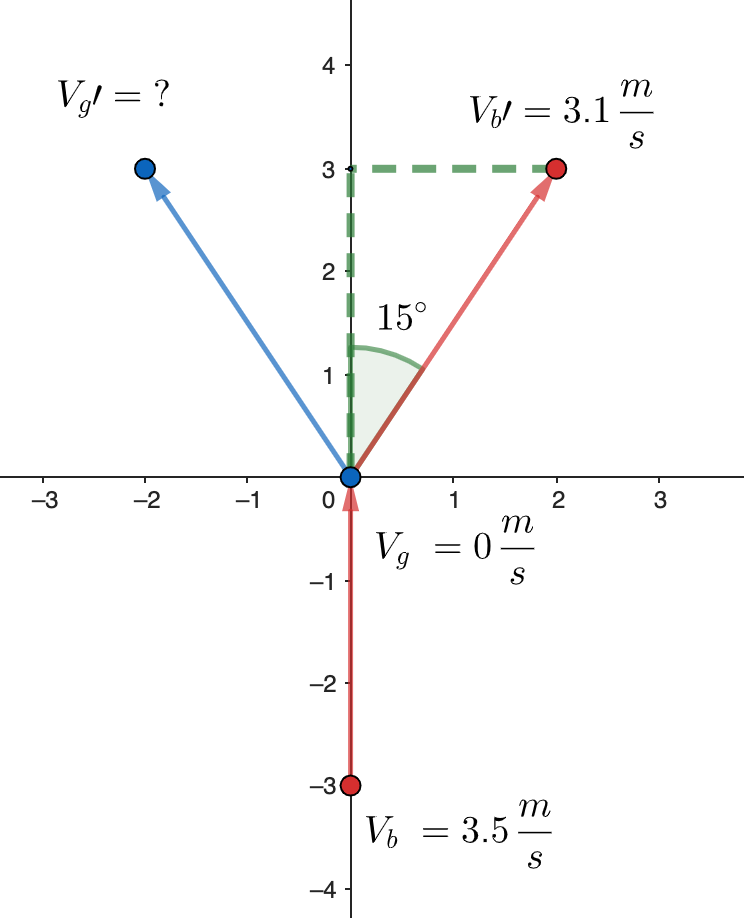
\includegraphics[scale=0.33]{./images/2d_momentum_graph}
    \end{minipage}
    \begin{minipage}{0.5\textwidth}
        \begin{itemize}
            \item $m_{b} = 0.155kg$
            \item $m_{g} = 0.052kg$
            \item $V_{b} = 3.5\frac{m}{s}$
            \item $V_{g} = 0\frac{m}{s}$
            \item $V_{b}\prime = 3.1\frac{m}{s}$ $[15\degree clockwise]$
            \item $V_{g}\prime = ?$
        \end{itemize}
    \end{minipage}
    \subsection*{2D Momentum - Solve for $v_{g}\prime$}
    \begin{adjustwidth}{1cm}{0pt}
        Since $v_{g}$ only has a $y$ direction, it's $x$ components are 0.\newline\newline
        $P_{tot_{x}} = P_{tot_{x}}\prime$ \\\\
        $(m_{g})(\cancel{v}_{g_{x}}^0) + (m_{b})(\cancel{v}_{b_{x}}^0) = (m_{g})(v_{g_{x}}\prime) + (m_{b})(v_{b_{x}}\prime)$ \\\\
        $\therefore v_{g_{x}}\prime = -\left(\frac{(m_{b})(v_{b_{x}}\prime)}{m_{g}}\right)$
        \\\\\\
        $P_{tot_{y}} = P_{tot_{y}}\prime$ \\\\
        $(m_{g})(\cancel{v}_{g_{y}}^0) + (m_{b})(v_{b_{y}}) = (m_{g})(v_{g_{y}}\prime) + (m_{b})(v_{b_{y}}\prime)$ \\\\
        $\therefore v_{g_{y}}\prime = -\left(\frac{(m_{b})(v_{b_{y}}) - (m_{b})(v_{b_{y}}\prime)}{m_{g}}\right)$
        \\\\\\
        $\therefore v_{g}\prime = \sqrt[]{{(v_{g_{y}}\prime)}^2 + {(v_{g_{x}}\prime)}^2}$ \\\\
    \end{adjustwidth}
\end{adjustwidth}


% make a diagram shwoign where Etot and Etot prime are and
% where Ptot and Ptot prime are. Recall the boulder diagram.
% do this in the equations area and use an equation for it
\end{document}